\section{Auswertung}
\label{sec:Auswertung}


\subsection{Ablenkung durch das E-Feld}

\subsubsection{Bestimmung der Apparaturkonstante}



Die Messwerte, welche zur Bestimmung der Empfindlichkeit des Ablenksystems benutzt werden, sind in Tabelle \ref{table:A2} dargestellt.
Dabei wird die Beschleunigungsspannung beginnend mit $U_{\text{B}} = \SI{200}{\volt}$ in $\SI{50}{\volt}$-Schritten erhöht.
\begin{table}
    \centering
    \caption{Messdaten zur Bestimmung der Ablenkung im E-Feld.}
    \label{table:b}
    \sisetup{parse-numbers=false}
    \begin{tabular}{
	S[table-format=1.2]
	S[table-format=4.2]
	S[table-format=4.2]
	S[table-format=4.2]
	S[table-format=4.2]
	S[table-format=4.2]
	}
	\toprule
	{$D \:/\: \text{in}$}		& {$U_1 \:/\: \si{\volt}$}		&
	{$U_2 \:/\: \si{\volt}$}		& {$U_3 \:/\: \si{\volt}$}		&
	{$U_4 \:/\: \si{\volt}$}		& {$U_5 \:/\: \si{\volt}$}		\\
	\midrule
    0.00 & -8.55 & -11.09 & -13.35 & -14.23 & -17.43 \\
0.25 & -4.58 & -6.36  & -7.82  & -7.67  & -10.13 \\
0.50 & -1.10 & -1.87  & -1.96  & -1.06  & -2.40  \\
0.75 & 2.61  & 2.91   & 3.79   & 5.38   & 5.17   \\
1.00 & 6.18  & 7.59   & 8.92   & 11.67  & 12.58  \\
1.25 & 9.59  & 12.00  & 14.64  & 17.93  & 19.83  \\
1.50 & 13.26 & 16.60  & 20.09  & 24.32  & 27.00  \\
1.75 & 16.80 & 20.98  & 25.31  & 30.78  & 34.23  \\
2.00 & 20.40 & 25.35  & 30.81  & /      & /      \\

    \bottomrule
    \end{tabular}
    \end{table}

Für jede Messreihe wird nun die Ablenkung $D$ gegen die Ablenkspannung aufgetragen.
Mittels linearer Ausgleichsrechnung wird die Steigung, welche der Empfindlichkeit $D/U$ entspricht, berechnet.
Dabei wird die Ausgleichsrechnung in Python mithilfe von SciPy \cite{scipy} durchgeführt.
\begin{table}
    \centering
    \caption{Fitparameter: Steigung $m$ und y-Achsenabschnitt $b$.}
    \label{tab:c}
    \sisetup{parse-numbers=false}
    \begin{tabular}{
	S[table-format=3.0]
	S[table-format=2.2]
	S[table-format=1.2]
	S[table-format=2.2]
	S[table-format=1.2]
	}
	\toprule
	{$U_b \:/\: \si{\volt}$}		& {$m \:/\: 10^{-4}\si{\metre\per\volt}$}		& 
	{$\increment{m} \:/\: 10^{-4}\si{\metre\per\volt}$}		& {$b \:/\: 10^{-3}\si{\volt}$}		& 
	{$\increment{b} \:/\: 10^{-3}\si{\volt}$}		\\ 
	\midrule
    17.67 & 0.08 & 14.68 & 0.09 \\
13.91 & 0.07 & 15.18 & 0.09 \\
11.51 & 0.06 & 15.11 & 0.10 \\
9.91  & 0.03 & 13.91 & 0.06 \\
8.58  & 0.04 & 14.84 & 0.08 \\

    \bottomrule
    \end{tabular}
    \end{table}

Die Fitparameter sind in Tabelle \ref{tab:c} angegeben, die entsprechenden Plots \ref{plot:1} bis \ref{plot:5} sind am Ende dieses Kapitels aufgeführt. \\
Werden diese Steigungen nun gegen die Reziproke der Beschleunigungsspannung aufgetragen ergibt sich der Plot \ref{plot:6}.
Über eine lineare Ausgleichsrechnung können die Fitparameter
\begin{align*}
  m &= \frac{pL}{2d} = \input{build/parameter_m6} \\
  b &= \input{build/parameter_b6}
\end{align*}
ermittelt werden, wobei die Steigung $m$ nach Formel \eqref{eqn:2} der zu bestimmenden Apparaturkonstante entspricht.

\begin{figure}
  \centering
  \includegraphics[height=6cm]{build/plot_a1.pdf}
  \caption{Plot zur Bestimmung der Empfindlichkeit bei $U_{\text{B}} = \SI{200}{\volt}$.}
  \label{plot:1}
\end{figure}

\begin{figure}
  \centering
  \includegraphics[height=6cm]{build/plot_a2.pdf}
  \caption{Plot zur Bestimmung der Empfindlichkeit bei $U_{\text{B}} = \SI{250}{\volt}$.}
  \label{plot:2}
\end{figure}

\begin{figure}
  \centering
  \includegraphics[height=6cm]{build/plot_a3.pdf}
  \caption{Plot zur Bestimmung der Empfindlichkeit bei $U_{\text{B}} = \SI{300}{\volt}$.}
  \label{plot:3}
\end{figure}

\begin{figure}
  \centering
  \includegraphics[height=6cm]{build/plot_a4.pdf}
  \caption{Plot zur Bestimmung der Empfindlichkeit bei $U_{\text{B}} = \SI{350}{\volt}$.}
  \label{plot:4}
\end{figure}

\begin{figure}
  \centering
  \includegraphics[height=6cm]{build/plot_a5.pdf}
  \caption{Plot zur Bestimmung der Empfindlichkeit bei $U_{\text{B}} = \SI{400}{\volt}$.}
  \label{plot:5}
\end{figure}

\begin{figure}
  \centering
  \includegraphics[height=6cm]{build/plot_a6.pdf}
  \caption{Plot zur Ermittlung der Apparaturkonstante.}
  \label{plot:6}
\end{figure}

\clearpage


\subsubsection{Untersuchung der Sinusspannung}
Bei der Untersuchung der Sinusspannung ergeben sich bei einer Beschleunigungsspannung von $U_b = \SI{400}{\volt}$ stehende Wellen für die folgenden Sägezahnfrequenzen:
\begin{align*}
  \nu_1 &= \input{build/v0.tex} \\
  \nu_2 &= \input{build/v1.tex} \\
  \nu_3 &= \input{build/v2.tex} \\
  \nu_4 &= \input{build/v3.tex}
\end{align*}
Es fällt auf, dass man bei einer Interpretation von $\nu_2$ als Grundfrequenz die Zuordnungen
\begin{align*}
  2\nu_1  &= \input{build/v0_mal_2.tex} \\
  \nu_2 &= \input{build/v1.tex} = \nu_\text{grund}\\
  \frac{1}{2}\nu_4 &= \input{build/v3_durch_2.tex}
\end{align*}
treffen kann, so dass die Sinusspannung $\nu_2$ beträgt.
Die Frequenz $\nu_3$ wird dabei jedoch ignoriert.
Nach Formel \eqref{eqn:2} ergibt sich für die Grundfrequenz eine dazugehörige Spannungsamplitude von
\begin{align*}
  \hat{U} &= \input{build/U_amp.tex}.
\end{align*}

\clearpage
\subsection{Ablenkung durch das B-Feld}
\subsubsection{Bestimmung der spezifischen Elektronenladung}
Bei den folgenden Messungen wird eine Helmholtzspule mit den Werten
\begin{align*}
  \mu_0 &= 4\pi \cdot 10^{-7}\si{\newton\per\ampere\tothe{2}},\\
  N    &= 20,\\
  R    &= \SI{0,282}{\metre} ,\\
  L    &= \SI{17,5}{\centi\metre} ,\\
\end{align*}
verwendet, wobei $N$ die Windungszahl und $R$ den Radius bezeichnet.
Zudem bezeichnet $L$ die Länge der verwendeten Kathodenröhre \cite{skript1} und $\mu_0$ die magnetische Feldkonstante.
Um die spezifische Elektronenladung zu ermitteln, wird, wie in der Durchführung beschrieben, die Ablenkung $D$ in Abhängigkeit von der an der Helmholtspule angelegten Stromstärke $I$ betrachtet.
Die Messergebnisse für die fünf verschiedenen Beschleunigungsspannungen, welche von $\SI{250}{\volt}$ bis $\SI{450}{\volt}$ in $\SI{50}{\volt}$-Schritten varriert werden, sind in Tabelle \ref{table:A2} angegeben.

\begin{table}
    \centering
    \caption{Messdaten zur Bestimmung der Ablenkung im B-Feld.}
    \label{table:A2}
    \sisetup{parse-numbers=false}
    \begin{tabular}{
	S[table-format=1.2]
	S[table-format=1.2]
	S[table-format=1.2]
	S[table-format=1.2]
	S[table-format=1.2]
	S[table-format=1.2]
	}
	\toprule
	{$D \:/\: \text{in}$}		& {$I_1 \:/\: \si{\ampere}$}		& 
	{$I_2 \:/\: \si{\ampere}$}		& {$I_3 \:/\: \si{\ampere}$}		& 
	{$I_4 \:/\: \si{\ampere}$}		& {$I_5 \:/\: \si{\ampere}$}		\\ 
	\midrule
    0.00 & 0.00 & 0.00 & 0.00 & 0.00 & 0.00 \\
0.25 & 0.28 & 0.30 & 0.32 & 0.35 & 0.40 \\
0.50 & 0.58 & 0.64 & 0.69 & 0.74 & 0.81 \\
0.75 & 0.89 & 1.00 & 1.07 & 1.14 & 1.25 \\
1.00 & 1.19 & 1.34 & 1.44 & 1.56 & 1.66 \\
1.25 & 1.52 & 1.68 & 1.81 & 1.94 & 2.09 \\
1.50 & 1.84 & 2.20 & 2.20 & 2.34 & 1.51 \\
1.75 & 2.18 & 2.39 & 2.58 & 2.75 & 2.94 \\
2.00 & 2.49 & 2.73 & 2.95 & /    & /    \\

    \bottomrule
    \end{tabular}
    \end{table}


Die Stärke des Magnetfeldes $B$, welches auf die Elektronen wirkt, berechnet mithilfe von
\begin{equation}
  B = \mu_0 \frac{8}{\sqrt{125}}\frac{N}{R} I
  \label{eqn:bfeld}
\end{equation}
aus der angelegten Stromstärke.
Dementsprechend folgen die Messergebnisse für $D$ in Abhängigkeit von $B$, die in Tabelle \ref{tab:d} angegeben sind.

\begin{table}
    \centering
    \caption{B-Feldstärken.}
    \label{tab:d}
    \sisetup{parse-numbers=false}
    \begin{tabular}{
	S[table-format=1.2]
	S[table-format=3.2]
	S[table-format=3.2]
	S[table-format=3.2]
	S[table-format=3.2]
	S[table-format=3.2]
	}
	\toprule
	{$D \:/\: \text{in}$}		& {$B_1 \:/\: \si{\micro\tesla}$}		& 
	{$B_2 \:/\: \si{\micro\tesla}$}		& {$B_3 \:/\: \si{\micro\tesla}$}		& 
	{$B_4 \:/\: \si{\micro\tesla}$}		& {$B_5 \:/\: \si{\micro\tesla}$}		\\ 
	\midrule
    0.00 & 0.00   & 0.00   & 0.00   & 0.00   & 0.00   \\
0.25 & 17.86  & 19.13  & 20.41  & 22.32  & 25.51  \\
0.50 & 36.99  & 40.81  & 44.00  & 47.19  & 51.65  \\
0.75 & 56.76  & 63.77  & 68.24  & 72.70  & 79.71  \\
1.00 & 75.89  & 85.45  & 91.83  & 99.48  & 105.86 \\
1.25 & 96.93  & 107.14 & 115.43 & 123.72 & 133.28 \\
1.50 & 117.34 & 140.30 & 140.30 & 149.23 & 96.29  \\
1.75 & 139.02 & 152.41 & 164.53 & 175.37 & 187.49 \\
2.00 & 158.79 & 174.10 & 188.13 & /      & /      \\

    \bottomrule
    \end{tabular}
    \end{table}


Zur Ermittlung der Konstante $\frac{e_0}{m_0}$ nach Formel \eqref{eqn:4} wird für jedes $U_\text{b}$ der Wert $\frac{D}{L^2+D^2}$ gegen $B$ aufgetragen.
Zudem wird ein linearer Fit mit SciPy durchgeführt.
Die Ergebnisse sind graphisch in den Abbildungen \ref{plot:7} bis \ref{plot:11} dargestellt, die Fitparameter sind in Tabelle \ref{tab:e} angegeben.

\begin{table}
    \centering
    \caption{Fitparameter: Steigung $m$ und y-Achsenabschnitt $b$.}
    \label{tab:e}
    \sisetup{parse-numbers=false}
    \begin{tabular}{
	S[table-format=3.0]
	S[table-format=4.2]
	S[table-format=3.2]
	S[table-format=1.2]
	S[table-format=1.2]
	}
	\toprule
	{$U_b \:/\: \si{\volt}$}		& {$m \:/\:\si{\per\metre\per\tesla}$}		& 
	{$\increment{m} \:/\:\si{\per\metre\per\tesla}$}		& {$b \:/\: \si{\per\metre}$}		& 
	{$\increment{b} \:/\:\si{\per\metre}$}		\\ 
	\midrule
    250 & 9597.92 & 207.87 & 0.05 & 0.02 \\
300 & 8585.09 & 212.44 & 0.05 & 0.02 \\
350 & 8086.01 & 149.22 & 0.04 & 0.02 \\
400 & 7745.58 & 128.28 & 0.03 & 0.01 \\
450 & 7275.21 & 102.05 & 0.02 & 0.01 \\

    \bottomrule
    \end{tabular}
    \end{table}


\begin{figure}
  \centering
  \includegraphics[height=6cm]{build/plot_a7.pdf}
  \caption{Plot zur Bestimmung des Proportionalitätsfaktors bei $U_{\text{B}} = \SI{250}{\volt}$.}
  \label{plot:7}
\end{figure}

\begin{figure}
  \centering
  \includegraphics[height=6cm]{build/plot_a8.pdf}
  \caption{Plot zur Bestimmung des Proportionalitätsfaktors bei $U_{\text{B}} = \SI{300}{\volt}$.}
  \label{plot:8}
\end{figure}

\begin{figure}
  \centering
  \includegraphics[height=6cm]{build/plot_a9.pdf}
  \caption{Plot zur Bestimmung des Proportionalitätsfaktors bei $U_{\text{B}} = \SI{350}{\volt}$.}
  \label{plot:9}
\end{figure}

\begin{figure}
  \centering
  \includegraphics[height=6cm]{build/plot_a10.pdf}
  \caption{Plot zur Bestimmung des Proportionalitätsfaktors bei $U_{\text{B}} = \SI{400}{\volt}$.}
  \label{plot:10}
\end{figure}

\begin{figure}
  \centering
  \includegraphics[height=6cm]{build/plot_a11.pdf}
  \caption{Plot zur Bestimmung des Proportionalitätsfaktors bei $U_{\text{B}} = \SI{450}{\volt}$.}
  \label{plot:11}
\end{figure}

Nach Formel \eqref{eqn:4} ergibt sich aus den Steigungen und den jeweiligen Beschleunigungsspannungen der Wert
\begin{equation}
  \frac{e_0}{m_0} = 8 U_\text{b} m^2.
\end{equation}
Hieraus folgen für die jeweligen Messreihen die Werte
\begin{align*}
  c_1 &= \input{build/konstante_0.tex} \\
  c_2 &= \input{build/konstante_1.tex} \\
  c_3 &= \input{build/konstante_2.tex} \\
  c_4 &= \input{build/konstante_3.tex} \\
  c_5 &= \input{build/konstante_4.tex}
\end{align*}
sowie gemittelt ein Wert von
\begin{align*}
  \frac{e_0}{m_0} &= \input{build/konstante_mean.tex}. \\
\end{align*}

%\clearpage

\subsubsection{Messung der Größe des Erdmagnetfeldes}
Zur Messung des Erdmagnetfeldes wird, wie in der Durchführung beschrieben, eine Kompensationsmessung durchgeführt.
Dabei ergibt sich, dass bei einem Strom von $I = \SI{0.26}{\ampere}$ das Erdmagnetfeld ausgeglichen wird, was nach Formel   \eqref{eqn:bfeld} einem Magnetfeld von
\begin{align*}
  B_\text{erd} &= \input{build/erdmagnetfeld.tex}
\end{align*}
entspricht.
Da ein endlicher Inklinationswinkel vorhanden ist, muss dieser zur Bestimmung der effektiven horizontalen Komponente berücksichtigt werden.
Dieser wird zu $\phi = \SI{70}{\degree}$ ermittelt, so dass sich der Wert
\begin{align*}
  \frac{B_\text{erd}}{\sin{(\phi)}} = B_\text{erd,korr} &= \input{build/erdmagnetfeld_korrigiert.tex}
\end{align*}
für die effektive Horizontalkomponente des Erdmagnetfeldes ergibt.

% % Examples
% \begin{equation}
%   U(t) = a \sin(b t + c) + d
% \end{equation}
%
% \begin{align}
%   a &= \input{build/a.tex} \\
%   b &= \input{build/b.tex} \\
%   c &= \input{build/c.tex} \\
%   d &= \input{build/d.tex} .
% \end{align}
% Die Messdaten und das Ergebnis des Fits sind in Abbildung~\ref{fig:plot} geplottet.
%
% %Tabelle mit Messdaten
% \begin{table}
%   \centering
%   \caption{Messdaten.}
%   \label{tab:data}
%   \sisetup{parse-numbers=false}
%   \begin{tabular}{
% % format 1.3 bedeutet eine Stelle vorm Komma, 3 danach
%     S[table-format=1.3]
%     S[table-format=-1.2]
%     @{${}\pm{}$}
%     S[table-format=1.2]
%     @{\hspace*{3em}\hspace*{\tabcolsep}}
%     S[table-format=1.3]
%     S[table-format=-1.2]
%     @{${}\pm{}$}
%     S[table-format=1.2]
%   }
%     \toprule
%     {$t \:/\: \si{\milli\second}$} & \multicolumn{2}{c}{$U \:/\: \si{\kilo\volt}$\hspace*{3em}} &
%     {$t \:/\: \si{\milli\second}$} & \multicolumn{2}{c}{$U \:/\: \si{\kilo\volt}$} \\
%     \midrule
%     \input{build/table.tex}
%     \bottomrule
%   \end{tabular}
% \end{table}
%
% % Standard Plot
% \begin{figure}
%   \centering
%   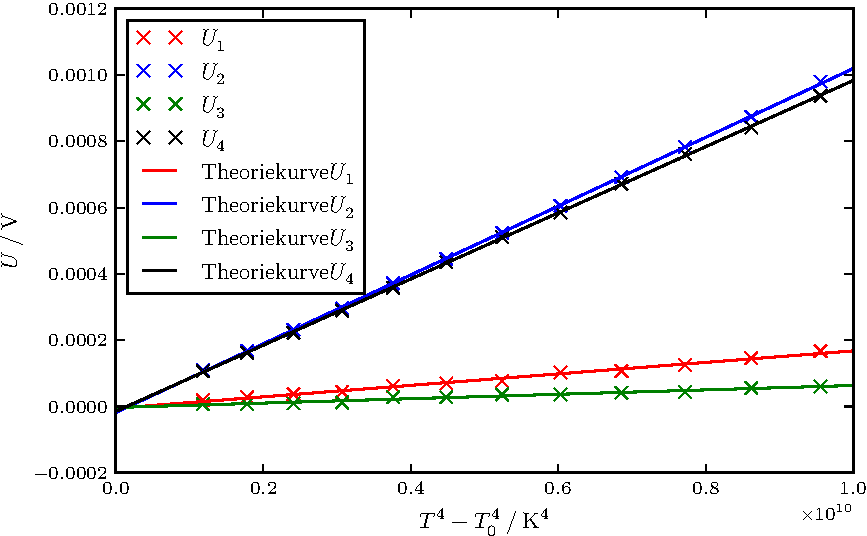
\includegraphics{build/plot.pdf}
%   \caption{Messdaten und Fitergebnis.}
%   \label{fig:plot}
% \end{figure}
%
% 2x2 Plot
% \begin{figure*}
%     \centering
%     \begin{subfigure}[b]{0.475\textwidth}
%         \centering
%         \includegraphics[width=\textwidth]{Abbildungen/Schaltung1.pdf}
%         \caption[]%
%         {{\small Schaltung 1.}}
%         \label{fig:Schaltung1}
%     \end{subfigure}
%     \hfill
%     \begin{subfigure}[b]{0.475\textwidth}
%         \centering
%         \includegraphics[width=\textwidth]{Abbildungen/Schaltung2.pdf}
%         \caption[]%
%         {{\small Schaltung 2.}}
%         \label{fig:Schaltung2}
%     \end{subfigure}
%     \vskip\baselineskip
%     \begin{subfigure}[b]{0.475\textwidth}
%         \centering
%         \includegraphics[width=\textwidth]{Abbildungen/Schaltung4.pdf}    % Zahlen vertauscht ... -.-
%         \caption[]%
%         {{\small Schaltung 3.}}
%         \label{fig:Schaltung3}
%     \end{subfigure}
%     \quad
%     \begin{subfigure}[b]{0.475\textwidth}
%         \centering
%         \includegraphics[width=\textwidth]{Abbildungen/Schaltung3.pdf}
%         \caption[]%
%         {{\small Schaltung 4.}}
%         \label{fig:Schaltung4}
%     \end{subfigure}
%     \caption[]
%     {Ersatzschaltbilder der verschiedenen Teilaufgaben.}
%     \label{fig:Schaltungen}
% \end{figure*}
